\documentclass{beamer}

\usetheme{Copenhagen}
\usepackage[utf8]{inputenc}
\usepackage{graphics}

% Slayt basliklarinda kullanilan font boyutu
\setbeamerfont{frametitle}{size=\normalsize}

\title{Resmin Şekillenmesi}
\author{Nurettin Şenyer}
\date{Şubat, 2011}
\institute[2011]{19/x}

\begin{document}

\frame{\titlepage}

\frame{\tableofcontents}

\frame {
	\frametitle {Önizleme}

	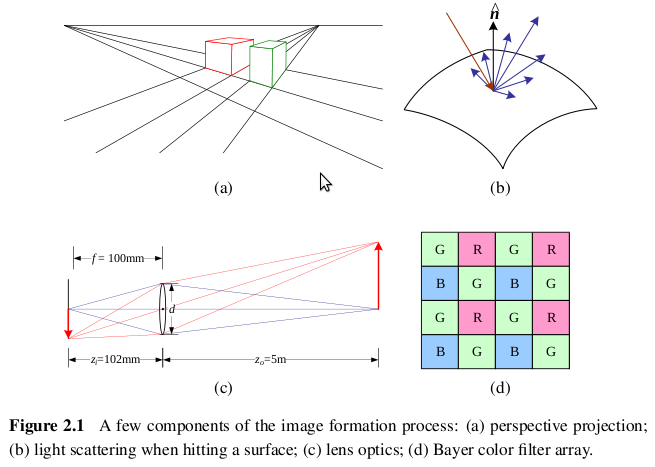
\includegraphics[width=0.95\textwidth]{img/fig21.png}
}

\section{Geometrik İlkeller ve Dönüşümler}

\frame {
	\frametitle {Giriş}

	Resmin şekillenişinde şu kavramlar önemli rol oynar

	\begin{itemize}
		\item ışıklanma koşulları
		\item sahnenin geometrisi
		\item yüzey özellikleri
		\item kamera optiği
	\end{itemize}
}

\subsection{Geometrik İlkeller}
\frame {
	\frametitle {Nokta}

	\begin{itemize}
		\item 2D düzlemde bir nokta: $\mathbf{x} = (x,y) \in R^2$

		\item Homojen karşılığı,
		$\mathbf{\widetilde{x}} = (\widetilde{x}, \widetilde{y}, \widetilde{z})	\in	P^2$

		\item Burada $P^2$ 2D yansıtma uzayı ve $P^2 = R^3 - (0,0,0)$

		\item inhomojen,
		\begin{eqnarray*}
			\mathbf{\widetilde{x}} &=& (\widetilde{x}, \widetilde{y}, \widetilde{z}) \\
									&=& \widetilde{w} \cdot (x,y,1) \\
									&=& \widetilde{w} \cdot \overline{x}
		\end{eqnarray*}

		\item burada $\overline{x} = (x,y,1)$ yardımcı (augmented) vektör

		\item Eğer $\widetilde{w} = 0$ ise ideal nokta (sonsuzdaki nokta) olarak adlanır ve
		inhomojen temsili yoktur
	\end{itemize}
}

\frame {
	\frametitle {2D Çizgi}

	$\overline{x} \cdot \widetilde{\l} = a \cdot x + b \cdot y + c = 0$

	Normalize etmek istersek: $\l = (\hat{\eta_x}, \hat{\eta_y}, d) =
	\mathbf{\hat{\eta}}, d)$ ve $||\mathbf{\hat{\eta}}|| = 1$ normal vektörüdür.

	\begin{columns}
		\column{0.5\textwidth}
		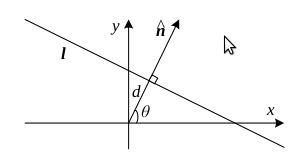
\includegraphics[width=0.95\textwidth]{img/fig22a.png}

		\column{0.5\textwidth}
		$\mathbf{\hat{\eta}}$, $\l$ doğrusuna merkezden $d$ uzaklığında dik
		olan vektördür.

		$\mathbf{\hat{\eta}} = (\hat{\eta_x}, \hat{\eta_y}) = (cos\theta,
		sint\theta)$ bu Hough dönüşümünde kullanılan temsildir.

		$(\theta, d)$ - polar gösterim
	\end{columns}
}

\frame {
	\frametitle {İki doğrunun kesişimi}

	\begin{itemize}
		\item iki doğrunun kesişimi: $\mathbf{\widetilde{x}} = \widetilde{\l_1}
		\times \widetilde{\l_2}$

		\item iki noktadan geçen doğru: $\widetilde{l} =
		\mathbf{\widetilde{x_1}} \times \mathbf{\widetilde{x_2}}$

		\item nokta veya doğru sayısı artınca "least square" yaklaşımı
	\end{itemize}
}


\frame {
	\frametitle {Koni}

	$\widetilde{x}^T \cdot W \widetilde{x} = 0$

	kamera kalibrasyonu ve multi-view geometride kullanılır
}

\frame {
	\frametitle {3D Nokta}

	\begin{itemize}
		\item $\mathbf{x} = (x,y,z) \in R^3$

		\item $\mathbf{\widetilde{x}} =
		(\widetilde{x},\widetilde{y},\widetilde{z}, \widetilde{w}) \in P^3$

		\item $\mathbf{\overline{x}} = (x,y,z,1)$

		\item $\mathbf{\widetilde{x}} = \widetilde{w} \cdot \mathbf{\overline{x}}$
	\end{itemize}
}

\frame {
	\frametitle {3D Düzlem}

	$\overline{x} \cdot \widetilde{m} = ax + by + cz + d = 0$

	Normalize edersek: $m = (\hat{\eta_x}, \hat{\eta_y}, \hat{\eta_z}, d) =
	(\mathbf{\hat{\eta}}, d)$ ve $||\mathbf{\hat{\eta}}|| = 1$

	\begin{columns}
		\column{0.5\textwidth}
			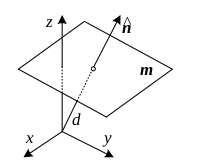
\includegraphics[width=0.95\textwidth]{img/fig22b.png}

		\column{0.5\textwidth}
			küresel koordinatlarla-$(\theta, \phi)$ tekrardan yazılabilir.

			$\mathbf{\hat{\eta}} = (cos\theta cos\phi, sin\theta cos\phi,
			sin\phi)$
	\end{columns}
}

\frame {
	\frametitle {3D Çizgi}

	$r = (1 - \lambda) p + \lambda q$ burada $0 \leq \lambda \leq 1$

	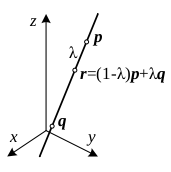
\includegraphics[height=0.85\textheight]{img/fig23.png}
}

\frame {
	\frametitle {3D Quadrik}

	Koninin 3D versiyonudur: $\overline{x}^T \cdot W \overline{x} = 0$
}

\subsection{2D Dönüşümler}
\frame {
	\frametitle {Önizleme}

	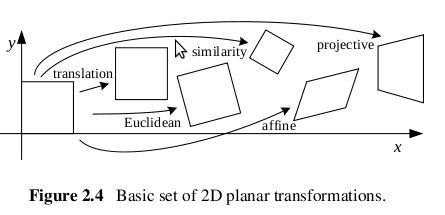
\includegraphics[width=0.95\textwidth]{img/fig24.png}
}

\frame {
	\frametitle {Kayma}

	$x' = x + t$

	$x' = [I_{2x2} | t] \cdot \overline{x}$

	$\overline{x'} =
		\begin{bmatrix}
		I & t\\
		0^T & 1
		\end{bmatrix} \cdot \overline{x}
	$ - augmented formdur
}

\frame {
	\frametitle {Dönme+Kayma}

	2D rigid body motion veya 2D Euclid dönüşümü: Euclid mesafesi korunduğundan

	$x' = Rx + t = [R | t] \overline{x}$

	burada $RR^T = I$ ve $|R|=1$

	$R = \begin{bmatrix}
			cos\theta & -sin\theta \\
			sin\theta & cos\theta
		 \end{bmatrix}$
}

\frame {
	\frametitle {Ölçekle+Döndür}

	Benzerlik dönüşümü: çizgiler arası açı korunduğundan

	$x' = sRx + t = [sR | t] \overline{x} 
		= \begin{bmatrix}
			a & -b & t_x \\
			b &  a & t_y
		  \end{bmatrix} \cdot \overline{x}
	$
}

\frame {
	\frametitle {Afin}

	$x' = A_{2x3} \cdot \overline{x}$

	burada $A$ keyfi değerlidir.

	Paralel çizgilerin paralelliği korunur.
}

\frame {
	\frametitle {Yansıtma}

	Perspective veya homography

	$\widetilde{x'} = \widetilde{H_{3x3}} \cdot \widetilde{x}$: homojen
	koordinatlar.

	$\widetilde{x'}$ den inhomojene şöyle geçilir, $\mathbf{x'} = (x', y')$

	$x' = \frac{h_{00}x + h_{01}y + h_{02}}{h_{20}x + h_{21}y + h_{22}}$
	$y' = \frac{h_{10}x + h_{11}y + h_{12}}{h_{20}x + h_{21}y + h_{22}}$

	Burada çizgi olma özelliği korunur.
}

\frame {
	\frametitle {Özet}

	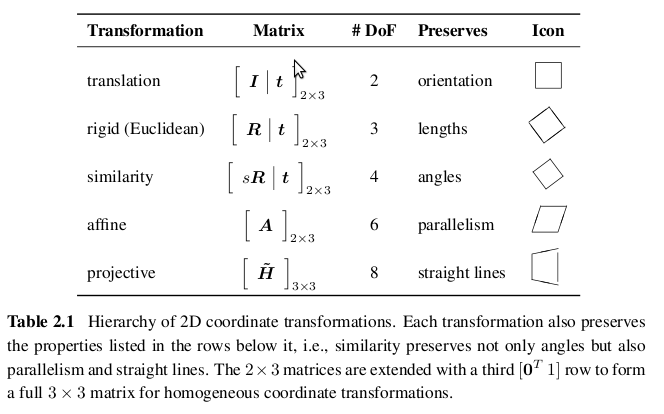
\includegraphics[width=0.95\textwidth]{img/table21.png}
}

\subsection{3D Dönüşümler}
\frame {
	3D dönüşümler, 2D'ye benzerdir ve önceki tabloda $2x3$ boyutları yerini
	$3x4$ ve $3x3$ boyutları da $4x4$'e bırakır.

	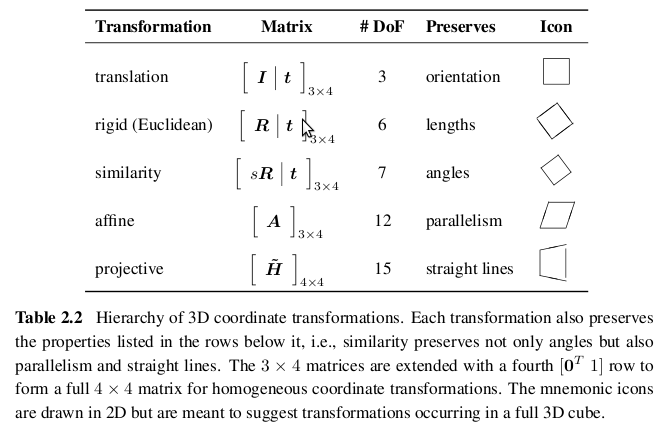
\includegraphics[width=0.90\textwidth]{img/table22.png}
}

\subsection{3D Döndürme}
\frame {
	\frametitle {Euler Açıları}
}

\frame {
	\frametitle {Eksen Açısı}

	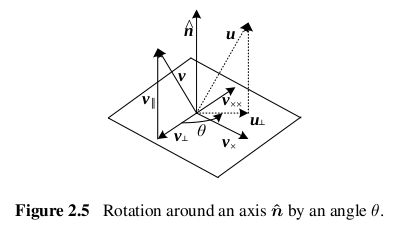
\includegraphics[width=0.90\textwidth]{img/fig25.png}
}

\frame {
	\frametitle {Birim Quaternion (Dördey)}

	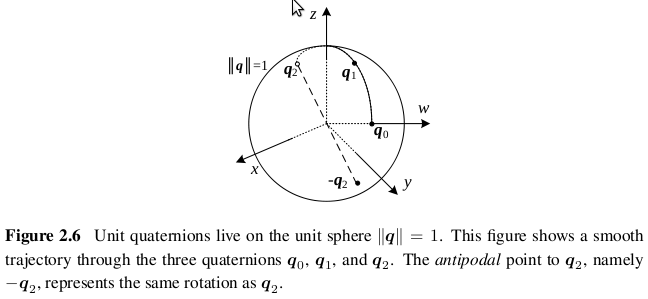
\includegraphics[width=0.90\textwidth]{img/fig26.png}
}

\frame {
	\frametitle {Hangi dönüşüm daha iyi?}
}

\subsection{3D'den 2D'ye Yansıtma}
\frame[allowframebreaks] {
	\frametitle {Önizleme}

	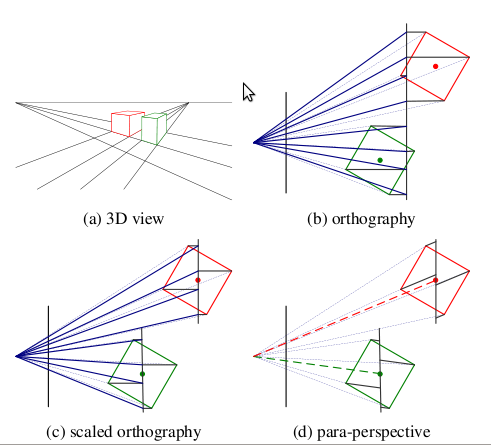
\includegraphics[width=0.90\textwidth]{img/fig27a-d.png}
	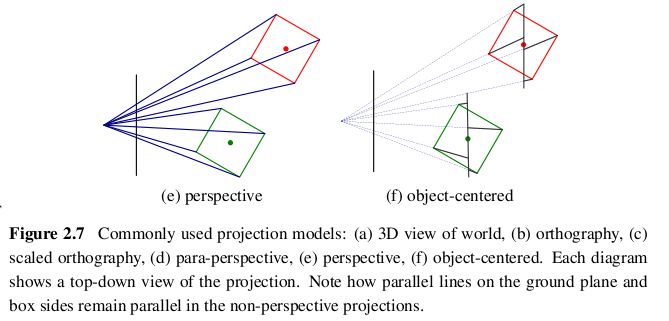
\includegraphics[width=0.90\textwidth]{img/fig27e-f.png}
}

\frame {
	\frametitle {Orthography ve Para-perspective}
}

\frame {
	\frametitle {Perspective}
}

\frame[allowframebreaks] {
	\frametitle {Kamera İçselleri (intrinsics)}

	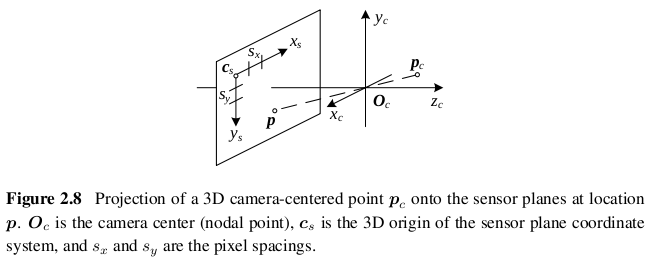
\includegraphics[width=0.90\textwidth]{img/fig28.png}
	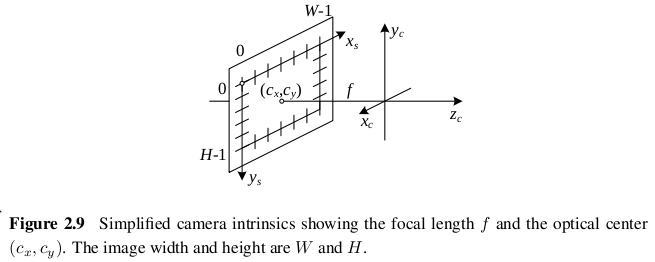
\includegraphics[width=0.90\textwidth]{img/fig29.png}
}

\frame {
	\frametitle {Odak Uzunluğu}

	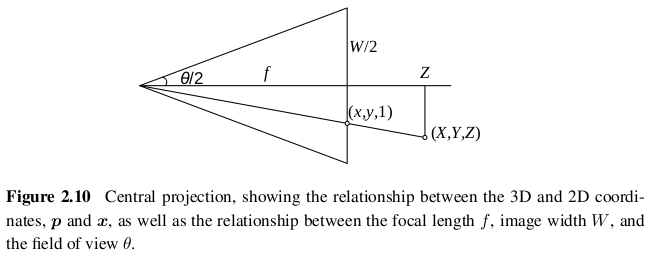
\includegraphics[width=0.90\textwidth]{img/fig210.png}
}

\frame {
	\frametitle {Kamera Matrisi}
}

\frame {
	\frametitle {Plane + Parallax (projective depth)}
}

\frame {
	\frametitle {Bir kameradan diğerine haritalama}

	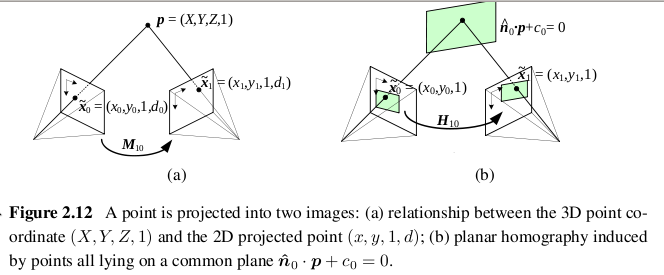
\includegraphics[width=0.90\textwidth]{img/fig212.png}
}

\subsection{Lens Bozulmaları}
\frame {
	\frametitle {A}

	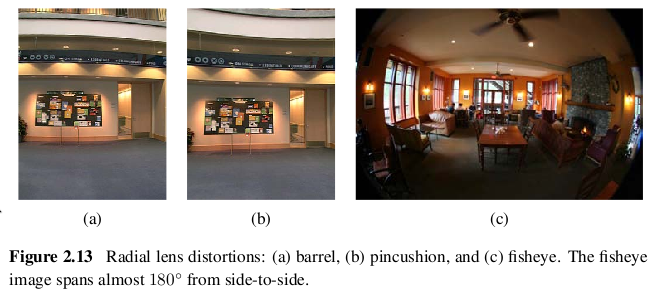
\includegraphics[width=0.90\textwidth]{img/fig213.png}
}

\section{Fotometrik Resim Şekillendirme}
\frame {
	\frametitle {A}

	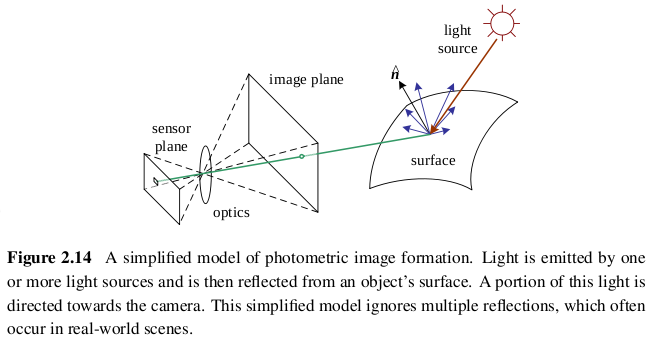
\includegraphics[width=0.90\textwidth]{img/fig214.png}
}

\subsection{Işıklanma}
\frame {
	\frametitle {A}
}

\subsection{Yansıma ve Gölgeleme}
\frame[allowframebreaks] {
	\frametitle {A}

	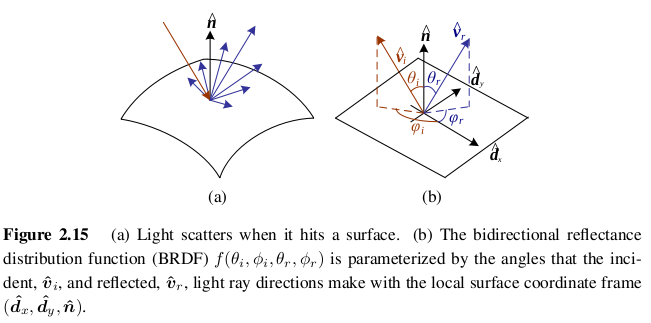
\includegraphics[width=0.90\textwidth]{img/fig215.png}
	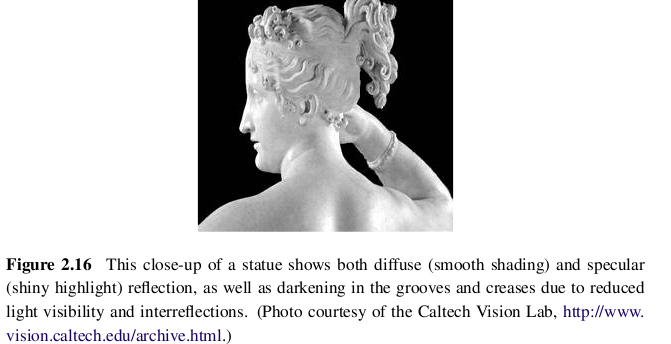
\includegraphics[width=0.90\textwidth]{img/fig216.png}
	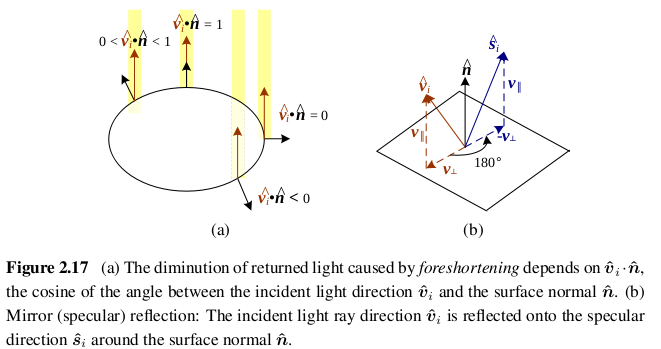
\includegraphics[width=0.90\textwidth]{img/fig217.png}
	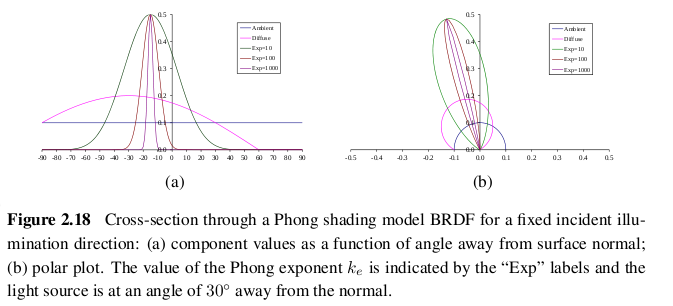
\includegraphics[width=0.90\textwidth]{img/fig218.png}
}

\subsection{Optik}
\frame[allowframebreaks] {
	\frametitle {A}

	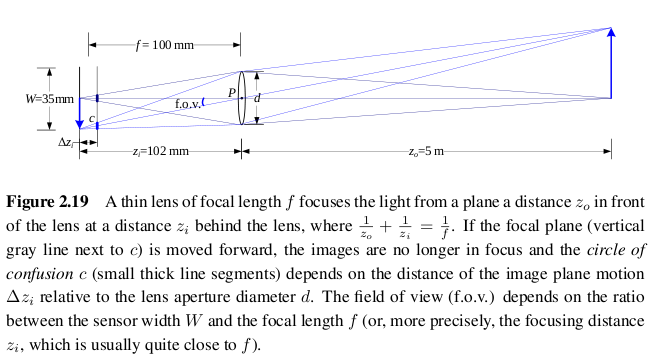
\includegraphics[width=0.90\textwidth]{img/fig219.png}
	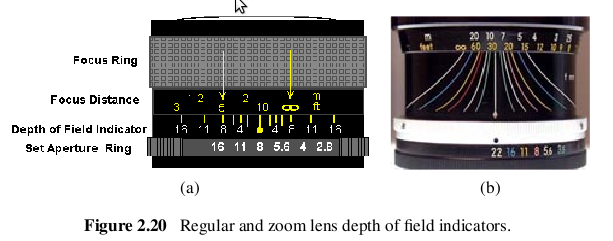
\includegraphics[width=0.90\textwidth]{img/fig220.png}
	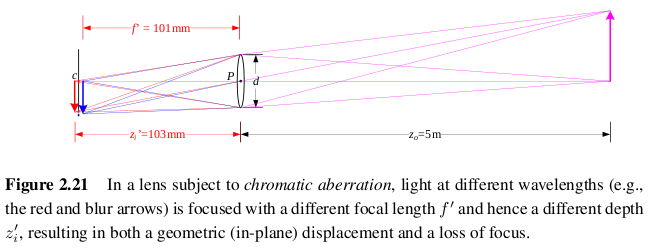
\includegraphics[width=0.90\textwidth]{img/fig221.png}
	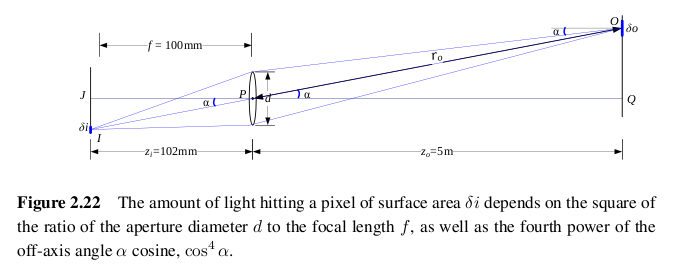
\includegraphics[width=0.90\textwidth]{img/fig222.png}
}

\section{Sayısal Kamera}
\frame {
	\frametitle {A}

	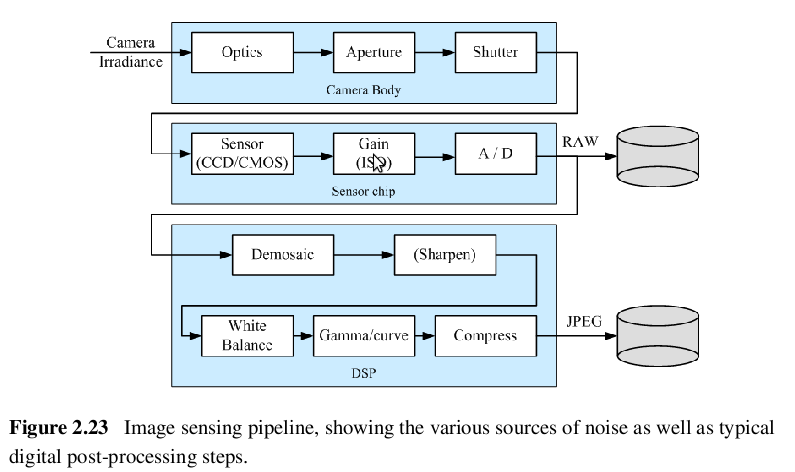
\includegraphics[width=0.90\textwidth]{img/fig223.png}
}

\subsection{Örnekleme ve Örtüşme}
\frame[allowframebreaks] {
	\frametitle {A}

	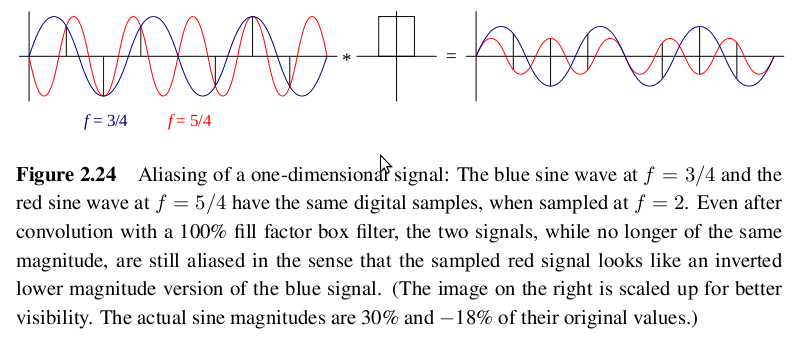
\includegraphics[width=0.90\textwidth]{img/fig224.png}
	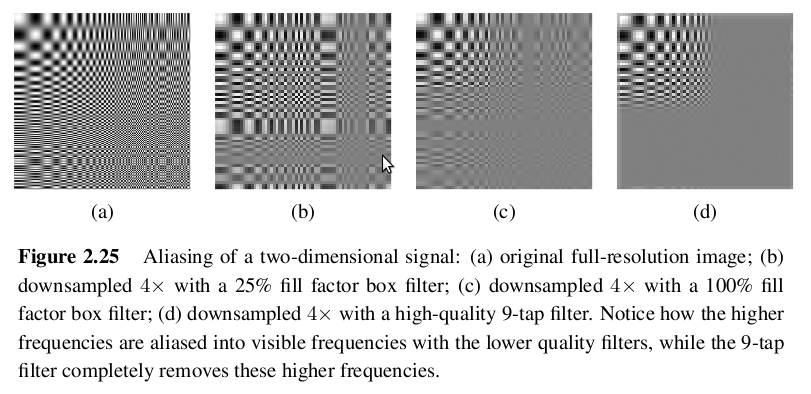
\includegraphics[width=0.90\textwidth]{img/fig225.png}
	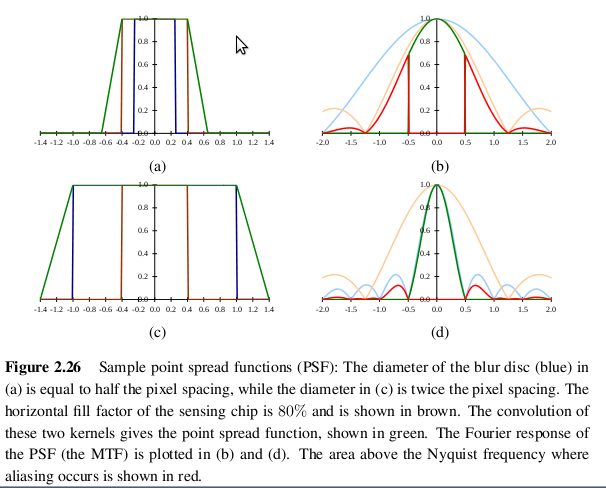
\includegraphics[width=0.90\textwidth]{img/fig226.png}
}

\subsection{Renk}
\frame[allowframebreaks] {
	\frametitle {A}

	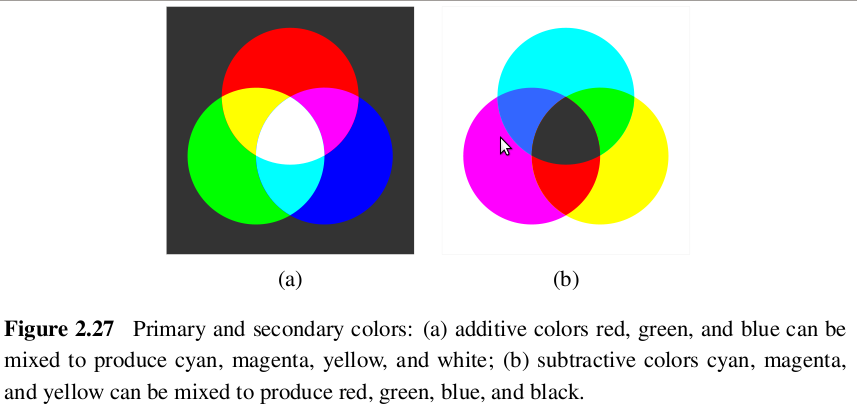
\includegraphics[width=0.90\textwidth]{img/fig227.png}
	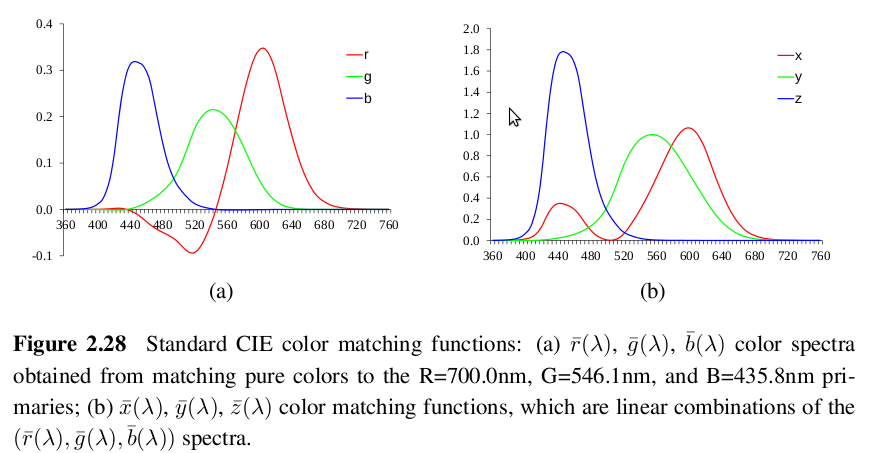
\includegraphics[width=0.90\textwidth]{img/fig228.png}
	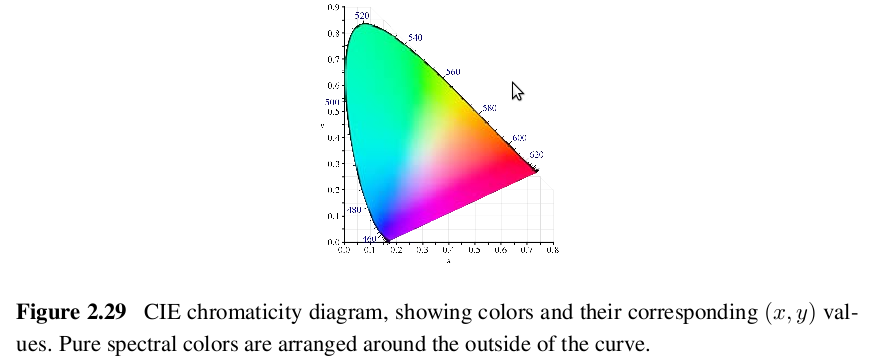
\includegraphics[width=0.90\textwidth]{img/fig229.png}
	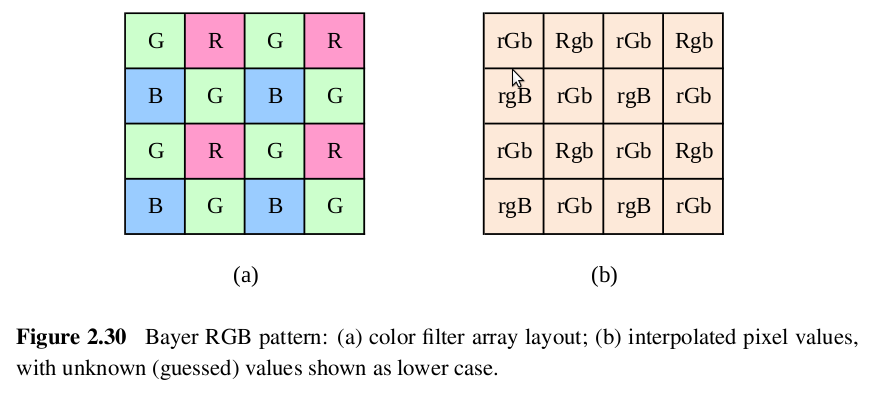
\includegraphics[width=0.90\textwidth]{img/fig230.png}
	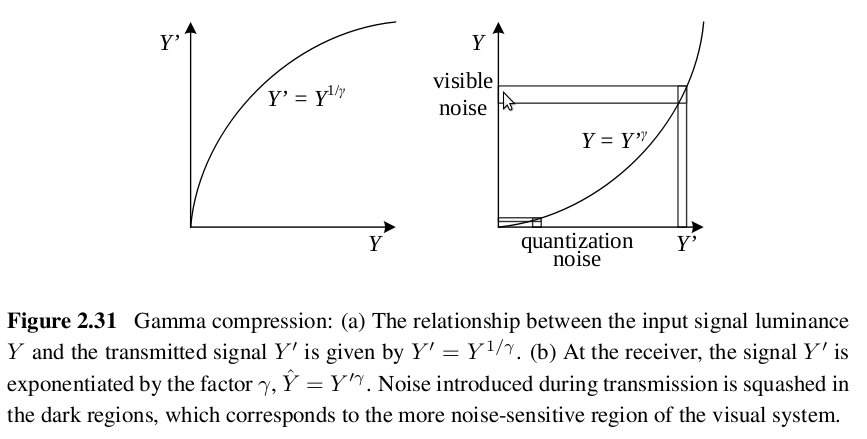
\includegraphics[width=0.90\textwidth]{img/fig231.png}
}

\subsection{Sıkıştırma}
\frame[allowframebreaks] {
	\frametitle {A}

	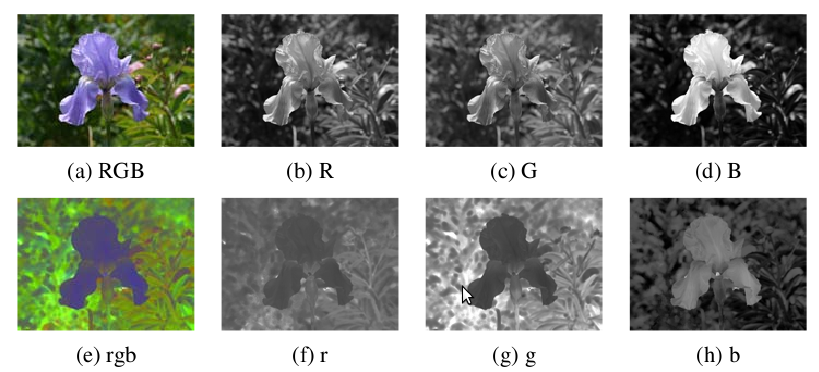
\includegraphics[width=0.90\textwidth]{img/fig232a-h.png}
	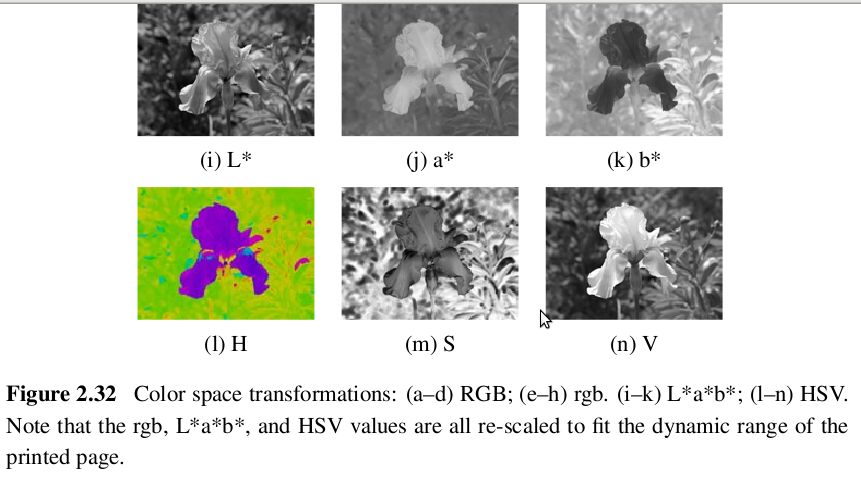
\includegraphics[width=0.90\textwidth]{img/fig232i-n.png}
	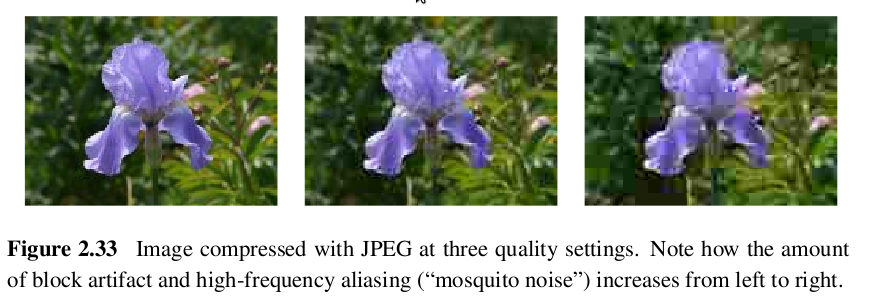
\includegraphics[width=0.90\textwidth]{img/fig233.png}
}

\end{document}
